% version 1.00	Auteur Pierre Porche

\documentclass[asi, sansVersion]{picInsa}

\usepackage{vocabulaireUnipik}
\usepackage{pdfpages}
\usepackage{graphicx}

\definecolor{gris}{gray}{0.75}
\definecolor{gris2}{gray}{0.85}

\titreGeneral{\FF}
\sousTitreGeneral{Base de Données}
\titreAcronyme{\FFCourt}
\version{}
\referenceVersion{\FFCourt\_Q\_\nomEquipe\_cArgoUml}
\auteurs{\Pierre{}}
\destinataires{\nomApprobateur{}, \nomTuteurQualite, \nomEquipe}
\resume{Le présent document est la \FF{} aux bases de données.}
\motsCles{\planQualite{}, PQ, PIC, \nomEquipe{}, \FF}
\natureDerniereModification{Création}
\modeDiffusionControle{}


\begin{document}

	\begin{center}
		\LARGE
		\textsc{
			\FF{}\\
			\No 02 - ArgoUML
		}
	\end{center}
	\vspace{0.5cm}

	\section*{Suivi des modifications}
		\begin{table}[H]
			\centering
			\begin{tabularx}{18cm}{|p{1.7cm}|X|p{4cm}|}
				\hline
				\rowcolor[gray]{0.90} Date & Nature de la modification \\
				\hline
				
				22/02/16 & Création \\
				\hline
			\end{tabularx}
		\end{table}

	\section*{Description}
		\begin{longtable}{|p{0.35\textwidth}|p{0.65\textwidth}|}
			\hline
			\cellcolor{gris2} Intitulé & Formation avancée aux bases de données\\\hline
			\cellcolor{gris2} Date de formation & 26/02/2016\\\hline
			\cellcolor{gris2} Date d'évaluation à chaud & 02/03/2016 \\\hline
			\cellcolor{gris2} Date d'évaluation à froid & 24/04/2016\\\hline
			\cellcolor{gris2} Démarche & Afin de maîtriser le logiciel ArgoUML, il a été nécessaire de former les membres de l'équipe.\\\hline
			\cellcolor{gris2} Évaluation &
				\textbf{Évaluation à chaud} : les membres de l'équipe ont répondu à un exercice noté par \Julie. La barre de validation a été fixée à 7 / 10.\newline
				\textbf{Évaluation à froid} : mise en œuvre des compétences acquises pour la réalisation du lot n°2.\\\hline
			\cellcolor{gris2} Évaluateurs & \Julie{}\\\hline
			\cellcolor{gris2} Membres évalués & \Pierre{}, \Melissa{}, \Sergi{}, \Michel{}, \Matthieu{}, \Mathieu{}, \Florian{}, \Kafui{}\\\hline
			\cellcolor{gris2} Membres reçus &  \\\hline
			\cellcolor{gris2} Supports & Les membres ont étudié les documents aux adresses : \begin{itemize}
			\item La documentation officielle (Partie 1.3.4 pour commencer) : \url{http://ftp.stu.edu.tw/BSD/FreeBSD/ports/distfiles/argouml/manual-0.34.pdf}
			\item Pour réaliser un diagramme de cas d'utilisation : \url{https://www.youtube.com/watch?v=U-sH0_rhgPU}
			\item Pour réaliser un diagramme d'activité : \url{https://www.youtube.com/watch?v=muoKDKQqFnc}
			\item Pour réaliser un diagramme de classe : \url{https://www.youtube.com/watch?v=BGM1QbPb9dQ}
			\item Pour réaliser un diagramme de séquence : Voir qualité/DSQ/FF/FRF/pdf/FRF\_Q\_Unipik\_cArgoUml\_n001.pdf
		\end{itemize}
			 \\\hline
			\cellcolor{gris2} Terminée & Non \\\hline
		\end{longtable}

	\newpage
	\section*{Évaluation à chaud}
		\subsection*{Exercices}
		Pour cette évaluation, vous ferez les exercices suivants : 
		\\
		
	%	\textbf{Exercice 1 :}\\
	%	Réaliser le diagramme d'activité suivant : 
	%	\includegraphics[scale=0.6]{diagrammeDActivite.png}
		\textbf{Exercice 1 :}\\
		Réaliser le diagramme d'activité suivant : \\
		\begin{figure}[H]
			\centering
			\includegraphics[scale=0.5]{images/diagrammeDActivite.png}
		\end{figure}			
		
		\textbf{Exercice 2 :}\\
		Réaliser le diagramme de classe suivant : \\
		\begin{figure}[H]
			\centering
			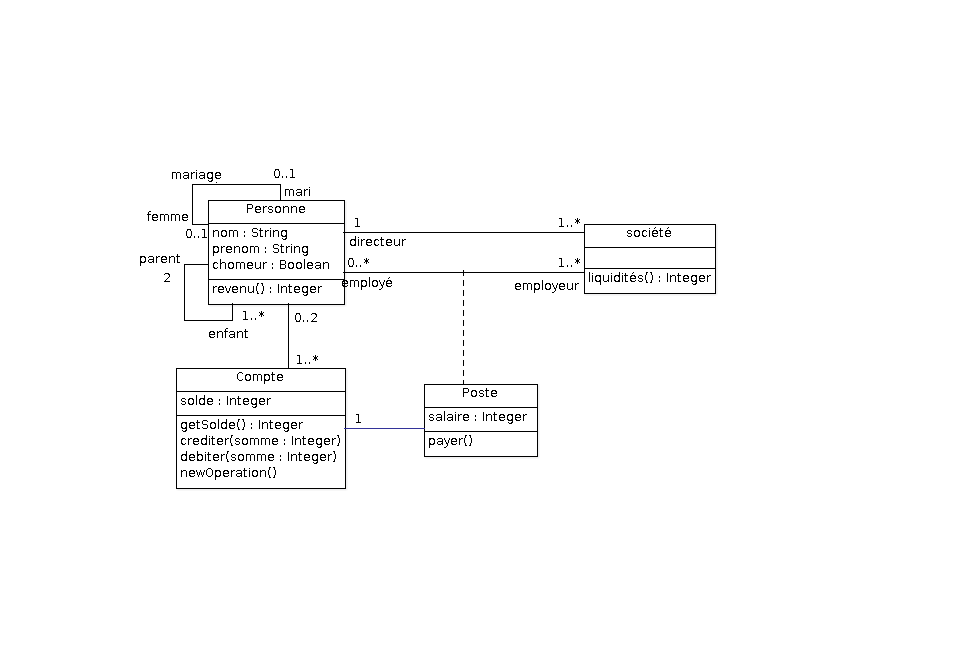
\includegraphics[scale=0.5]{images/diagrammeDeClasse.png}
		\end{figure}
		
		\textbf{Exercice 3 :}\\
		Réaliser le diagramme de cas d'utilisation : \\
		\begin{figure}[H]
			\centering
		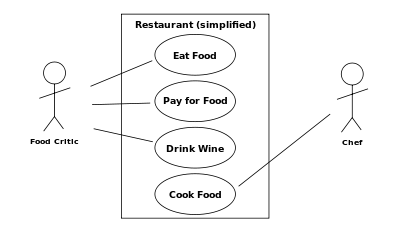
\includegraphics[scale=1]{images/diagrammeDeCasDUtilisation.png}
		\end{figure}
			
			\vspace{8px}
			
		\subsection*{Résultats}
			\begin{longtable}{|p{0.5\textwidth}|p{0.5\textwidth}|}
				\hline
					\rowcolor[gray]{0.90} Nom & Note (/10) \\
				\hline
					\Sergi & 9.5 \\
				\hline
					\Pierre & 10 \\
				\hline
					\Mathieu & 9.5 \\
				\hline
					\Michel & 10 \\
				\hline
					\Matthieu & 9.5 \\
				\hline
					\Kafui & 9 \\
				\hline
					\Melissa & 9 \\
				\hline
					\Florian & 9 \\
				\hline
			
			\end{longtable}
			
	\newpage
	\section*{Évaluation à froid}
		L'évaluation à froid correspond à la réalisation des documents de conception.

\end{document}
